\documentclass[conference]{IEEEtran}
\IEEEoverridecommandlockouts
\usepackage{cite}
\usepackage{amsmath}
\usepackage{amssymb}
\usepackage{amsfonts}
\usepackage{algorithmic}
\usepackage{graphicx}
\usepackage{textcomp}
\usepackage{xcolor}
\usepackage{graphicx}
%% \usepackage{subfigure}
\usepackage{subfig}
%% \usepackage{subcaption}
\def\BibTeX{{\rm B\kern-.05em{\sc i\kern-.025em b}\kern-.08em
    T\kern-.1667em\lower.7ex\hbox{E}\kern-.125emX}}
\begin{document}
\title{Photovoltaic System Reconfiguration strategy for mismatch condition\\
{\footnotesize \textsuperscript{}}}

\author{\IEEEauthorblockN{1\textsuperscript{st} Dafang Zhao}
\IEEEauthorblockA{\textit{dept. name of organization (of Aff.)} \\
\textit{name of organization (of Aff.)}}
\and
\IEEEauthorblockN{2\textsuperscript{nd} Given Name Surname}
\IEEEauthorblockA{\textit{dept. name of organization (of Aff.)} \\
\textit{name of organization (of Aff.)}}
\and
\IEEEauthorblockN{3\textsuperscript{rd} Given Name Surname}
\IEEEauthorblockA{\textit{dept. name of organization (of Aff.)} \\
\textit{name of organization (of Aff.)}}}

\maketitle

\begin{abstract}
  Power generation efficiency of photovoltaic(PV) system is reduced significantly under partial shading or solar cell damage  conditions. This efficiency losses affected by truing on bypass diode of PV panels, which called mismatch losses. Reconfiguration technology to reconfigure electrical series or parallel connection among PV panel can maximize generate power. This paper proposes a reconfiguration strategy that finds an optimal configuration among mismatched PV array in a less computational time. This algorithm is very light and suitable for embedded device. The results show that compare with existed reconfiguration method under non-uniform shadow scenario proposed algorithm computes an optimized configuration with less computational time and very high accuracy.
\end{abstract}

\begin{IEEEkeywords}
  Photovoltaic system, mismathed power loss, reconfiguration, dynamical reconfiguration.
\end{IEEEkeywords}

\section{Introduction} \label{intro}

As the world of fossil energy constantly exhausted and the increasingly serious environmental pollution, the research and utilization of renewable and green energy have become necessary means of survival and development of human being. Photovoltaic (PV) energy has received a significant attention since it is unlimited and easy to be scaled up. Thanks to extensive technology and research on photovoltaic energy generation, large scale photovoltaic energy generation systems have been deployed into many practical applications. However, PV arrays are sensitive to shading and PV cell's fault or aging. This implies that when interconnection of PV cells or modules do not have identical properties or experience different conditions from one another. the PV array is in mismatch condition. The photovoltaic arrays under mismatched conditions will accelerate the aging and heating of PV cells and cause a short circuit of photovoltaic cells to further damage the PV array. In order to avoid mismatch condition damage PV cells, we propose an algorithm that can reconfigure photovoltaic arrays to avoid mismatch damage and maximize generated power.

In this paper, we use non-uniform irradiance levels to represent mismatch condition and analyze the efficiency of a PV system under different shaded working condition. Photovoltaic arrays operating in non-uniform irradiance levels may present multiple local maximum power points (MPPs) \cite{b1}, which are generated by turning on bypass diodes. By changing electrical connection among the panels to prevent activate bypass diodes is a recent appealing solution\cite{b2}.

The main difficulty facing the reconfiguration problem is that some or even all panels can be subjected to partial shading and there may be more than one MPP for each panel. Moreover, the panels, and not modules, reconfiguration strategy has to be realized so that modules providing the highest power could be grouped separately\cite{b3} \cite{b4}.

This procedure enables to detect panel's operating conditions, in more than two-strings, receiving different irradiance levels. The reconfiguration algorithm will analyzes panels' working conditions and reorganizes panels into different strings by different irradiance levels. However, in sparse of mismatching conditions, distribution of panels among different irradiance levels are not significant. For that, by increasing number of strings in the PV array and using exhaustive search can be a solution\cite{b3}. Another approach to optimize photovoltaic arrays is using genetic algorithm\cite{b5}. However, computing cost is too significant, and this algorithm can't detect best configuration precisely. A simplest reconfiguration strategy for minimizing mismatch losses is presented in \cite{b10}. In this strategy, an algorithm gives candidates for PV array reconfiguration, for each candidates we have conduct power simulations. But some candidates are not feasible, which means there isn't any configuration for PV array can be realized. Since the power simulation is very time consuming, based on existed work we want to reduce number of candidates to accelerate overall reconfiguration algorithm. In this paper we propose an algorithm can give optimal configuration and check feasibility with less computational time and high accuracy.  

\section{Assumption of a PV array} \label{assum}
In this paper, we use the following definitions of PV arrays, modules, strings and panels as showed in Fig. \ref{fig1}. A PV array is formed by several parallel connected (PV) strings, and a string is formed by several series-connected PV panels. For a PV panel, formed by three PV modules connected in series with bypass diodes. 
\begin{figure}[htbp]
\centerline{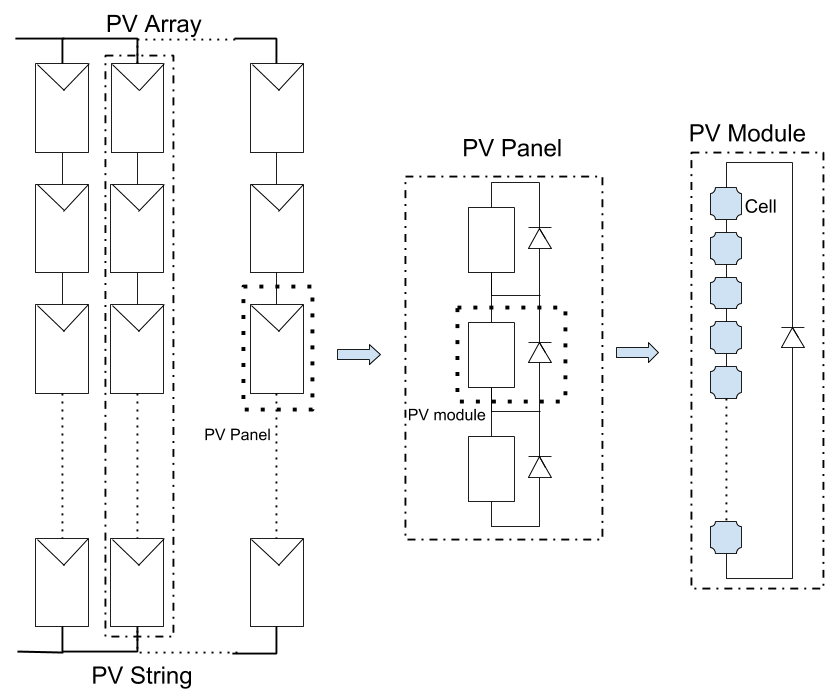
\includegraphics[width=7.2cm]{paper-fig1.png}}
\caption{PV arrays, strings, and panels.}
\label{fig1}
\end{figure}

We assume that each panel follows: The current versus voltage (\textit{I-V}) curve is acquired and calculated by algorithm presented in \cite{b6}. That algorithm will analyzes the panel \textit{I-V} curve sample by finding almost-constant-current and voltage regions and coordinate multiple maximum or minimum power point in the \textit{P-V} curve if PV array is working in mismatched conditions or not. 

All the panels in PV array have the same number (\textit{N}) of modules. For particular module, using (\textit{$V_{mpp_n}$, $I_{mpp_n}$}) to identify voltage and current values on different maximum power point by index \textit{n}. Those parameters can be directly estimated by the prosess provided in\cite{b7}.


Furthermore, it is also assumed that for each string it has same number of panels. Means every string in PV array have same length. String's length are identical based on when they connected in parallel, a string has more panels may cause current back flow into other strings which have less panels\cite{b8}.
\begin{figure}[htbp]
\centerline{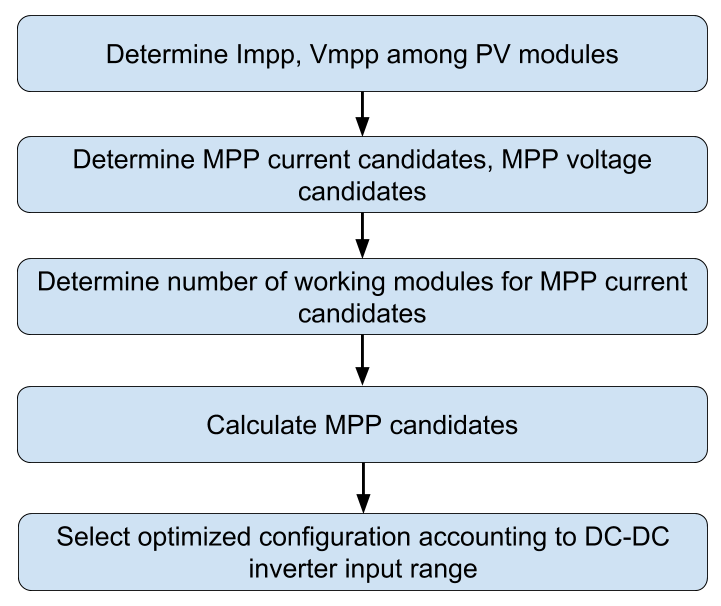
\includegraphics[width=8cm]{flowchart.png}}
\caption{Flowchart of reconfiguration algorithm in \cite{b10}.}
\label{flowchart}
\end{figure}


\section{Reconfiguration Algorithm} \label{algo}
As described in \cite{b10}, the Fast reconfiguration strategy firstly determine \textit{$V_{mpp}$} and \textit{$I_{mpp}$} for each PV module by using the algorithm in \cite{b7} \cite{b9}. Then determine MPP current and voltage candidates among PV array. Calculate MPP candidates matrix by multiplying the current and voltage candidates. Using the number of working modules (\textit{$Q_{M_n}$}) for each MPP current candidates to determine MPP candidates. Finally the Fast reconfiguration strategy gives MPP candidates for reconfiguration, which specifies a current value and minimum number of working modules for each string in PV array. Due to a PV panel can not be used into different string, those MPP candidates may have some un-feasible configurations. The general steps of Fast reconfiguration strategy as showed in Fig. \ref{flowchart}.

\subsection{Feasibility}
The feasibility of configuration based on the assumption of section \ref{assum}, each string in PV array must have same number of panels. Definition of feasibility in (\ref{feas}). When a configuration needs panels in a string (\textit{$NP_n$}) are over mean value for number of panels per-string this configuration is unfeasible. 
\begin{equation}
\left\{\begin{matrix}
NP_n > NP\div N_{st}& & \text{Unfeasible}\\ 
NP_n \leq NP\div N_{st} & & \text{Feasible} 
\label{feas}
\end{matrix}\right. 
\end{equation}

\begin{table}[htbp]
\caption{}
\begin{center}
\begin{tabular}{cccc}
\multicolumn{4}{c}{DATA OF PARTIAL-SHADING PV ARRAY} \\ \hline \hline
Panels & Vmpp(V)                & Impp (A)            & MPP(W)                 \\ \hline
P1     & {[}0, 2.9, 11.4{]}     & {[}0, 0.5, 2{]}     & {[}0, 1.5, 22.8{]}     \\
P2     & {[}2.9, 17.1, 17.1{]}  & {[}0.5, 3, 3{]}     & {[}1.5, 51.3, 51.3{]}  \\
P3     & {[}2.9, 2.9, 2.9{]}    & {[}0.5, 0.5, 0.5{]} & {[}1.5, 1.5, 1.5{]}    \\
P4     & {[}0, 11.4, 11.4{]}    & {[}0, 2, 2{]}       & {[}0, 22.8, 22.8{]}    \\
P5     & {[}0, 2.9, 11.4{]}     & {[}0, 0.5, 2{]}     & {[}0, 1.5, 22.8{]}     \\
P6     & {[}2.9, 11.4, 11.4{]}  & {[}0.5, 2, 2{]}     & {[}1.5, 22.8, 22.8{]}  \\
P7     & {[}2.9, 11.4, 17.1{]}  & {[}0.5, 2, 3{]}     & {[}1.5, 22.8, 51.3{]}  \\
P8     & {[}11.4, 11.4, 11.4{]} & {[}2, 2, 2{]}       & {[}22.8, 22.8, 22.8{]} \\
P9     & {[}2.9, 11.4, 17.1{]}  & {[}0.5, 2, 3{]}     & {[}1.5, 22.8, 51.3{]} 
\end{tabular}
\label{tab1}
\end{center}
\end{table}

\subsection{Reconfiguration strategy}
Based on existed reconfiguration
%The general steps of reconfiguration algorithm are presented in Fig. \ref{fig2}. The first step is determine each PV module's \textit{$V_{mpp}$} and \textit{$I_{mpp}$} by using algorithm provided in \cite{b7} \cite{b9}, and calculate MPP current and voltage candidates of PV array. When there are more than two panels connected in series, for a string MPPs is not straightforward. The MPP current and voltage candidates can be evaluated though a procedure presented in \cite{b10}. For string MPP current candidates, \textit{$I_{mpp_n}$} values' different less than 5\% are assumed to be equal. For string MPP voltage candidates, \textit{$V_{mpp_n}$}  can be calculated though multiplay number of active modules (\textit{$N_a$}) by average MPP voltages (\textit{$\bar V_{mpp}$}) with $\pm$18\% error \cite{b10}. Afterward, determine real number of working modules (\textit{$Q_{M_n}$}) for each MPP current candidates by applying method in \cite{b10}. Next, find MPP candidates by multiplying current candidates and voltage candidates which determine by \textit{$Q_{M_n}$}. Due to \textit{$V_{mpp}s$} and \textit{$I_{mpp}s$} can indicate shading distribution among PV array.  Then grouping panels into different shadow distribution.  

After this procedures is conducted for PV array, all panels will be organized into many groups that from un-shadowed or uniform shadow to fully shadowed group. However, if just simply grouping panels by shadow distribution conditions it may cause electrical connection overhead or unable calculate optimal configuration. To further reconfigure PV system into a better configuration, the replacement part of algorithm will proceed as follow:
\begin{itemize}
\item Sorting group by different shadow distribution conditions, select panels from first group into a PV string which working on high current level.
\item If selected panels' working modules ( \textit{$Q_{M_n}^{*}$} ) less than \textit{$Q_{M_n}$} , select panels from next irradiance level group.
\item If selected panels' \textit{$Q_{M_n}^{*}$} more than \textit{$Q_{M_n}$}, re-select panels to adjust \textit{$Q_{M_n}^{*}$} equal to \textit{$Q_{M_n}$} if it is possible. 
\end{itemize}
\begin{figure}[htbp]
\centerline{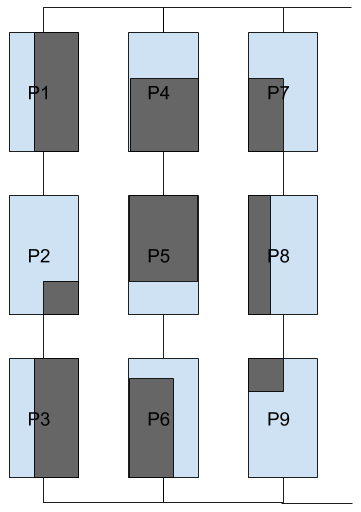
\includegraphics[width=6.2cm]{paper-fig3.png}}
\caption{An example of un-uniform shadowed PV array.}
\label{fig3}
\end{figure}

This algorithm will better understood by applying to shadow condition showed in Fig. \ref{fig3}. This PV system is composed with 9 PV panels connected into 3 strings as showed in Fig.\ref{fig3}. Irradiance levels, \textit{$I_{mpp}$} and \textit{$V_{mpp}$} of each module are given in Table \ref{tab1}. 

%\begin{table}[]
%\begin{tabular}{cccc}
%\multicolumn{4}{c}{Data of partial-shading PV array} \\
%\\ \hline \hline
%Panels   & Vmpp(V)  & Impp (A)             & MPP(w)  \\ \hline
%P1       &          & {[}0, 0.5, 2{]}      &         \\
%P2       &          & {[}0.5, 3, 3{]}      &         \\
%P3       &          & {[}0.5, 0.5, 0.5{]}  &         \\
%P4       &          & {[}0, 2, 2{]}        &         \\
%P5       &          & {[}0, 0.5, 2{]}      &         \\
%P6       &          & {[}0.5, 2, 2{]}      &         \\
%P7       &          & {[}0.5, 2, 3{]}      &         \\
%P8       &          & {[}2, 2, 2{]}        &         \\
%P9       &          & {[}0.5, 2, 3{]}      &        
%\end{tabular}
%\end{table}



The example refer to a three-strings PV array, each string contain with 3 panels, each one made of three identical PV modules (\textit{N}=3). In this example, it is assumed that input range of DC-DC converter and MPPT device defined by \textit{$V_{min}$} = 200V and \textit{$V_{max}$} = 500V. MPP current candidates and MPP voltage candidates are present in ( \ref{e1} ) and ( \ref{e2} ), respectively. Additional, number of real working module at MPP current candidates are given in ( \ref{e3} ).
\begin{equation}
\begin{aligned}
\textit{$I_{mpp_n}$} = [&\{  \text{$0.5_{(9)}$}, \text{$0.5_{(9)}$}, \text{$0.5_{(9)}$}   \}, \{ \text{$0.5_{(9)}$}, \text{$0.5_{(9)}$}, \text{$2_{(11)}$} \},  \\ &\{\text{$0.5_{(9)}$}, \text{$0.5_{(9)}$}, \text{$3_{(4)}$} \}, \{\text{$0.5_{(9)}$}, \text{$2_{(11)}$}, \text{$2_{(11)}$} \}, \\ & \{\text{$0.5_{(9)}$}, \text{$2_{(11)}$}, \text{$3_{(4)}$} \}, \{\text{$0.5_{(9)}$}, \text{$3_{(4)}$}, \text{$3_{(4)}$} \}, \\ &\{\text{$2_{(11)}$}, \text{$2_{(11)}$}, \text{$2_{(11)}$} \}, \{\text{$2_{(11)}$}, \text{$2_{(11)}$}, \text{$3_{(4)}$} \}, \\ & \{\text{$2_{(11)}$}, \text{$3_{(4)}$}, \text{$3_{(4)}$} \}, \{\text{$3_{(4)}$}, \text{$3_{(4)}$}, \text{$3_{(4)}$} \}] \pm 5\%  \label{e1}
\end{aligned}
\end{equation}
\begin{equation}
\begin{aligned}
\textit{$V_{mpp_n}$} = [&12.4, 24.8, 37.2, 49.6, 62.0, 74.4, 86.8, 99.2, \\&111.6] \pm 18\% \label{e2}
\end{aligned}
\end{equation}
\begin{equation}
\begin{aligned}
\textit{$Q_{M_n}$} = [&\{8,8,8\}, \{8,8,8\}, \{4,4,4\}, \{7,7,7\}, \{4,4,4\}, \\&\{2,2,2\}, \{5,5,5\}, \{4,4,4\}, \{2,2,2\}, \{1,1,1\}] \label{e3}
\end{aligned}
\end{equation}
 
\begin{figure}[htbp]
\centerline{
\includegraphics[width=8cm]{paper-fig4.png}}
\caption{Organized PV array after first part of Algorithm.}
\label{fig4}
\end{figure}

Due to 5\% error of MPP current candidates and 18\% error of MPP voltage candidates, total error rate of MPP candidates is 23\%. Though procedure of algorithm, MPP candidates with 23\% are: [\{ 0.5, 0.5, 2\}, \{0.5, 2, 2\}, \{2, 2, 2\}, \{2, 2, 3\}] and require working modules per strings are: [\{8, 8, 8\}, \{7, 7, 7\}, \{5, 5, 5\}, \{4, 4, 4\}]. And PV array are organized as Fig.\ref{fig4}
Those MPP candidates are able to generate maximum output power of PV system, but the configurations of MPP candidates may meet electrical connection overhead. In order to reduce electrical connection simulation time, replacement and feasibility check will be approved. 

Consider fourth MPP candidate, it require panels on string one working at 2A, panels on string two working at 2A, panels on string three working at 3A and require 4 PV modules working for each string. Firstly, selecting panels for high current string, string three. According to Table \ref{tab1}, only Panel 2, Panel 7 and Panel 9 are able to work at 3A. Those four panel can provide 4 PV module working at 3A and meet requirement of \textit{$Q_{M_n}$}. Because on extra panel can provide module  working on 3A, no replacement will be approved. Means no further improvement for configuration of string three.
Then select panel for string two, Panel 4 and Panel 8 will be selected, but this configuration is not optimized. Selected panels provide 5 modules able to work at 2A, satisfy requirement of \textit{$Q_{M_n}$} $\ge$ 4, but one module more than requirement. The process will replace Panel 4 by Panel 1 that provide just 4 modules working at 2A. Configuration for string two are Panel 8 and Panel 1. At last, select panels for string one. Panel 4, Panel 5, Panel 6 are selected, they can provide 5 modules working at 2A that satisfy requirement. For configuration on string one due to it is the last string to process and meet requirement, in order to reduce computing time replacement will not be approved. Configuration of MPP candidate \{2, 2, 3\} are \textit{St} 1:\{Panel 4,Panel 5, Panel 6\}, \textit{St} 2: \{Panel 1, Panel 8\}, \textit{St} 3: \{Panel 2, Panel 7, Panel 9\}. As described in section \ref{assum}, each string have identical length and Panel 3 not been used in any configuration. So optimized configuration for this MPP candidate are: \textit{St} 1:\{Panel 4,Panel 5, Panel 6\}, \textit{St} 2: \{Panel 1, Panel 8, Panel 3\}, \textit{St} 3: \{Panel 2, Panel 7, Panel 9\}. The MPP values of this configuration calculated by multiplay string voltage and current equal to 347.2W are put into evidence. 

For the third MPP candidate, as same calculating procedure as fourth MPP candidate, optimized configuration for MPP candidate \{2, 2, 2\} are: \textit{St} 1:\{Panel 4,Panel 8, Panel 3\}, \textit{St} 2: \{Panel 1, Panel 2, Panel 6\}, \textit{St} 3: \{Panel 5, Panel 7, Panel 9\}. 

The first MPP candidate \{0.5, 0.5, 2\}, after replacement string three contain four panels, \{Panel 4, Panel 8, Panel 1, Panel 2\} but it is over maximum string length of this PV array.
Also for MPP candidate \{0.5, 2, 2\}, there are no configuration can't provide 7 modules working 
on three different string at 0.5A, 2A, 2A, respectively. 

\section{evaluation of optimization algorithm}
%\subsection{Verification of the Proposed algorithm}
This section verifies the effectiveness of proposed algorithm using LTspice simulation. With pilot example presented in last section, shading scenario as showed in Fig.\ref{fig5a}. To minimize power loss, the proposed algorithm, as described, is applied to reconfigure the system. The resulting configuration is depicted in Fig.\ref{fig5b} and Fig.\ref{fig5c}. 
\begin{figure}
\centering
 
\subfloat[]{
	\label{fig5a}
	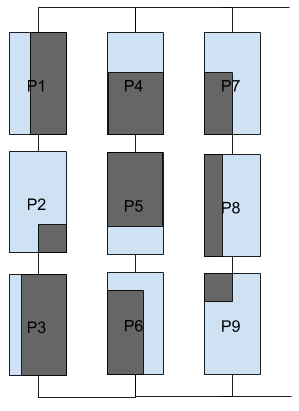
\includegraphics[width=5cm]{paper-fig5(a).png} } \\
\subfloat[]{
	\label{fig5b}
	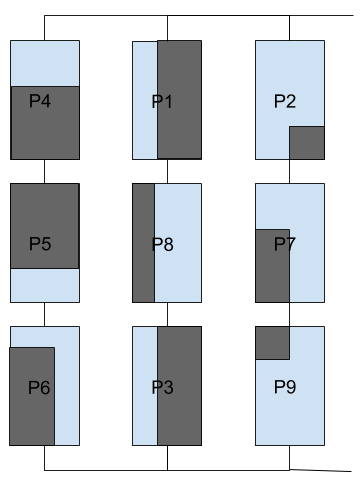
\includegraphics[width=5cm]{paper-fig5(b).png} } \\
\subfloat[]{
	\label{fig5c}
	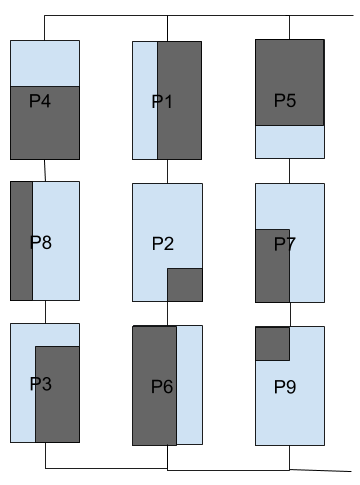
\includegraphics[width=5cm]{paper-fig5(c).png}} \\
\caption{The PV system under shading scenario (a) before reconfiguration, (b) after reconfiguration for MPP candidate \{2, 2, 3\} and (c) MPP candidate \{2, 2, 2\}} 
\end{figure}

%% \begin{figure}[htbp]            
%% \begin{minipage}[t]{0.5\linewidth}
%% \centerline{
\includegraphics{fig2.png}}
%% \caption{(a)}
%% \label{fig5a}
%% %\end{minipage}%
%% %\begin{minipage}[t]{0.5\linewidth}
%% \centerline{
\includegraphics{fig2.png}}
%% \caption{(b)}
%% \label{fig5b}
%% \end{minipage}
%% \end{figure}

As shown, working module on each string are large or equal than required \textit{$Q_{M_n}$}, which means mismatched power loss are minimized. The \textit{P-V} curve for this PV array before and after reconfiguration are showed in Fig.\ref{fig6}. It can be seen that after reconfiguration maximum power (!!!!!!!!!! W and !!!!!!W) are significantly higher than before reconfiguration maximum power (!!!!!!!!W).

\begin{figure}[htbp]
\centerline{
\includegraphics[width=6.2cm]{fig2.png}}
\caption{The \textit{P-V} curves for the PV system under first shading scenario before and after reconfiguration.}
\label{fig6}
\end{figure}
The computational time required to find the best configuration in the proposed and existed method is also compared and summarized in Table \ref{tab2}. As shown in Table \ref{tab3}, proposed algorithm achieved high accuracy and less computing time compare with exhaustive search algorithm and methods described in \cite{b10} \cite{b11} \cite{b12}.

\begin{table}[htbp]
\caption{}
\begin{center}
\begin{tabular}{ccc}
\multicolumn{3}{c}{\begin{tabular}[c]{@{}c@{}}COMPARISON BETWEEN EXISTED METHODS \\ AND PROPOSED ALGORITHM\end{tabular}} \\ \hline
Methods                                     & Computational time  & Accuracy  \\ \hline
The method in \cite{b10}   &                     &           \\
The method in \cite{b11}   &                     &           \\
The method in \cite{b12}   &                     &           \\
Exhaustive search Algorithm                 &                     &           \\
Proposed Algorithm                          &                     &          
\end{tabular}
\label{tab2}
\end{center}
\end{table}

%The simulations were performed using an Intel i7-4770 3.2-Ghz processor with 32.0 GB of RAM memory. 
The calculation time used by the proposed algorithm was !!!!! ms, which is significantly lower compared with exhaustive search (!!!!!!!time) and accuracy are much higher than methods proposed in \cite{b11} \cite{b12}.
\section{conclusions}
The existing PV reconfiguration methods either have high accuracy but suffer from long computational time such as exhausted searching algorithm or GA, or they have short computational time but do not guarantee the best configuration as described in \cite{b10} \cite{b11} \cite{b12}. This paper proposed a new PV system reconfiguration algorithm with high accuracy and less computational time. Proposed algorithm's effectiveness has been validated using LTspice simulation. The algorithm was tested though un-uniform shadow distribution among PV array and shows its effectiveness in finding optimal configuration. The proposed algorithm also compared with existed method in terms of accuracy and computational time. The result shows that proposed algorithm has high accuracy and less computational time.

\begin{thebibliography}{00}
\bibitem{b1} Koutroulis, Eftichios, and Frede Blaabjerg. "A new technique for tracking the global maximum power point of PV arrays operating under partial-shading conditions." IEEE Journal of Photovoltaics 2.2 (2012): 184-190.
\bibitem{b2} La Manna, Damiano, et al. "Reconfigurable electrical interconnection strategies for photovoltaic arrays: A review." Renewable and Sustainable Energy Reviews 33 (2014): 412-426.
\bibitem{b3}Storey, Jonathan, Peter R. Wilson, and Darren Bagnall. "The optimized-string dynamic photovoltaic array." IEEE Transactions on Power Electronics 29.4 (2014): 1768-1776.
\bibitem{b4} Storey, Jonathan P., Peter R. Wilson, and Darren Bagnall. "Improved optimization strategy for irradiance equalization in dynamic photovoltaic arrays." IEEE transactions on power electronics 28.6 (2013): 2946-2956.
\bibitem{b5} P. Carotenuto, A. D. Cioppa, A. Marcelli, and G. Spagnuolo, “An evolu- tionary approach to the dynamical reconfiguration of photovoltaic fields,” Neurocomputing, vol. 170, pp. 393–405, 2015.
\bibitem{b6} Carotenuto, Pietro Luigi, et al. "Online recording a PV module fingerprint." IEEE Journal of Photovoltaics 4.2 (2014): 659-668.
\bibitem{b7} Orozco-Gutierrez, M. L., et al. "Fast estimation of MPPs in mismatched PV arrays based on lossless model." Clean Electrical Power (ICCEP), 2015 International Conference on. IEEE, 2015.
\bibitem{b8} Spagnuolo, Giovanni, et al. "Control of photovoltaic arrays: Dynamical reconfiguration for fighting mismatched conditions and meeting load requests." IEEE Industrial Electronics Magazine 9.1 (2015): 62-76.
\bibitem{b9} Carotenuto, Pietro Luigi, et al. "Online recording a PV module fingerprint." IEEE Journal of Photovoltaics 4.2 (2014): 659-668.
\bibitem{b10} Orozco-Gutierrez, M. L., et al. "Optimized configuration of mismatched photovoltaic arrays." IEEE J. Photovolt 6.5 (2016): 1210-1220.
\bibitem{b11} El-Dein, MZ Shams, Mehrdad Kazerani, and M. M. A. Salama. "Optimal photovoltaic array reconfiguration to reduce partial shading losses." IEEE Trans. Sustain. Energy 4.1 (2013): 145-153.
\bibitem{b12} Storey, Jonathan P., Peter R. Wilson, and Darren Bagnall. "Improved optimization strategy for irradiance equalization in dynamic photovoltaic arrays." IEEE transactions on power electronics 28.6 (2013): 2946-2956.
  
\end{thebibliography}
\end{document}
